% $Id: solution.tex 
% !TEX root = ../main.tex

\section{Flik: A Bugs Life Debugger}
\label{sec:solution}

The black box behavior of \ac{ML} and \ac{RL} agents posit a problem to understand agents and 
their behavior, especially if unexpected behavior is observed. We posit debuggers as an appropriate 
tool to understand agents' behavior. Moreover, we posit debuggers with the possibility to modify 
programs' state and continue execution using new execution paths are even more appropriate and 
suitable to understand \ac{RL} agents, given their intrinsic nature of continuous interaction with the 
environment. However, currently, there is no debugger for \ac{RL} programs with the desired 
features. The reason for this is that most of the debuggers are postmortem, or do not allow developers
to go back in time to replay and analyze the program state. Additionally, most of the debuggers do not 
allow developers to modify variables. In order to contribute to the development of \ac{RL} programs, 
debugging tools should exhibit the following features:

\begin{description}
    \item[Stepping back:] Due to the execution loop of \ac{RL} programs, we 
    want to have a functionality that will allow us to step back the execution to observe the change 
    in state between iterations of the loop. This will let developers interacting directly with the program, 
    without having to stop the execution,  lose the program state, or the training data already 
    accumulated. Such feature will help in identifying the root cause of erroneous agent behavior, 
    whether that is an error in the program's design for particular interactions, or an ill-defined 
    hyperparameter. 
    \item [Modifying variables:] While stepping back into the program's execution, we would want to be 
    able to modify variables' values during the execution. Such feature would help to test out the 
    behavior of an agent with different state-values, or hyperparameters, without having to 
    continuously stop and retrain the agent, which can be very costly and time-consuming. 
\end{description}

These features aim at tackling the problem of interaction with the program, as it allows 
to inspect the behavior of a program with respect to different variable values. Additionally, 
developers may interact with the program execution by going forward and backward, observing the 
effects of specific interactions between the agent and the environment. The capacity to explore the 
execution (backward and forward) would allow for the evaluation of the behavior and quality of 
\ac{RL} programs, helping to improve the development of these programs.

With these features in mind, we present \flik: \textsc{A bugs life}, a back-in-time debugger with the 
possibility to step back in the execution, change values for different variables, and resume execution 
on different execution paths. \flik is not a traditional debugger; it is valuable to debug \ac{RL} 
programs, allowing to evaluate the internal state of the agent, the decisions it makes, and the rewards 
it receives, through the observation of its variables over time. Using the debugger, developers can 
better understand the execution context of \ac{RL} agents in terms of variables, values, environment, 
states and the rewards. 

\flik is a console-based debugger, constructed over the \ac{PDB} debugger. \flik adds features 
such as colored syntax highlighting, tracking of variables' state, and capturing stdout output 
from executed lines of code. The following are the three major features of \flik:
\begin{itemize}
    \item Stores the state in each execution step (\ie action taken by the agent). \flik saves the local 
    and global variables, in a history variable. Additionally, other metadata like the information of the 
    line being executed is saved. This allows us to later step back into specific states in the stored 
    history, and their corresponding location in the code. 
    \item Restores a previous program state as, from the previously stored information, from the 
    stack and heap variables to precisely restore the program's state and its execution context, in 
    order to re-create an alternative execution path. 
    \item Finally, connecting the previous two features, is the action of stepping back. This feature is 
    created as a custom \ac{PDB} command, using the same syntax and form of the native \ac{PDB} 
    commands. The stepping back command takes the state saved at a specific point in the history 
    and restores the state according to the information at that point --that is, program's state, stack 
    information, and code line. 
\end{itemize}

In Python, the internal state of a program during execution is primarily encapsulated in 
stack frames. Each stack frame contains information about the execution state of a function 
call, including the current line number, local and global variables, and other metadata, as follows:
\begin{itemize}
    \item \spy{f_lineno}: The current line number being executed.
    \item \spy{f_locals}: A dictionary of local variables within the frame.
    \item \spy{f_globals}: A dictionary of global variables accessible within the frame.
    \item \spy{f_code}: A code object representing the function's bytecode and source code metadata.
\end{itemize}

The state is saved in a list that stores snapshots of the frame's state (line and variables) at each 
execution step, which allows stepping back into any state we would want to restore. We use the  
\spy{exec} function that receives the stored \spy{f_globals} and \spy{f_locals} variables as 
parameters. \spy{exec} then executes a list of stored state snapshots (line number 
and local variables) at each step in a specified frame's context (given by the function parameters). 
This allows \flik to simulate running a specific line in the context of a previous frame, maintaining 
both local and global variable references, essentially restoring the saved execution state.

This all done by extending the \ac{PDB} class and adding custom commands to support stepping 
back and a custom interface which allows the user to interact with the debugger. The interface 
displays the code, variables, and execution point, and allows the user (to use the \ac{PDB} 
functions) to pause, step forward, step back, continue or restart the program, as well as to 
modify and inspect variables. 

\fref{fig:debugger} shows \flik's interface on a simple example of the \spy{bubble_sort} function. From 
the top, the first frame (in the blue rectangle Execution frame) we have the running execution, in this 
case the print for the array to be sorted in Line 18 in the second frame. The second frame (in the 
purple rectangle Source code frame) shows the source code that is being debugged. The third frame 
(in the red rectangle Variables frame) shows the variables used in the program so far. Finally, in the 
bottom of the interface we have the interactive console in which developers can send commands to 
\flik to effectively debug the program.

\begin{figure}[hptb]
    \centering
    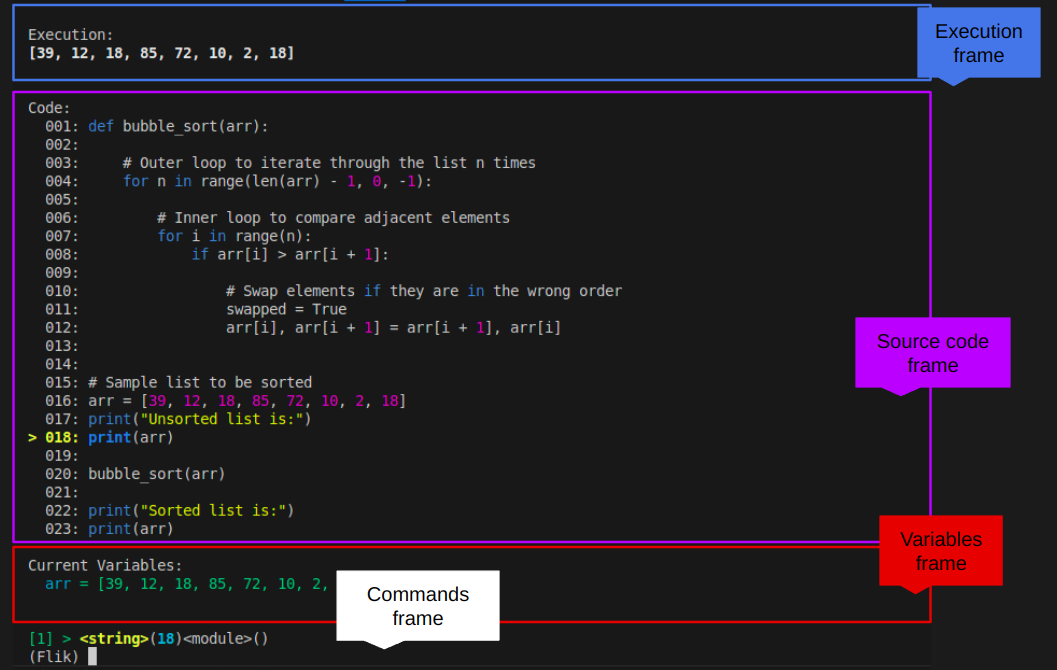
\includegraphics[width=0.9\textwidth]{figures/flik_interface.png}
    \caption{Debugger tool}
    \label{fig:debugger}
\end{figure}

We now use a running example to present the features, commands and inner work of \flik. Four 
our running example we use the GridWorld \ac{RL} benchmark. The environment consists of a 
$10 \times 10$ grid, shown in \fref{fig:gridworld}. The agent can move in four directions: up, down, 
left, and right at every GridWorld cell. However, the movement is not successful in bordering cells 
or cells adjacent to walls (\ie gray-out cells), as it collides with the walls and bounces back to the 
starting position.
The agent's reward is defined obtaining a reward of 1 when the agent gets to the goal state, and a 
reward of -1 when the agent visits trap states, terminating the execution in both cases. The agent 
starts in a fixed position, the top left corner of the grid (the blue state in \fref{fig:gridworld}). 

For the purpose of the running example, we will use the Q-learning implementation of the GridWorld 
agent as shown in \fref{lst:gridworld-learner}, explaining the \flik commands used to detect a bug in 
the code. Running the program, we pay special attention to the \spy{run} function, which we can 
access using the \spy{n} command until we reach it. Alternatively, it is possible to move directly to a 
specific execution point, by setting breakpoints in the program. For example, when executing the 
program, we can use the \spy{c} command to execute until the \spy{breakpoint} in \fref{ln:breakpoint} 
is reached. Once in the function, we use the \spy{n} command to step through the function. 
At particular points in the execution (\eg \fref{ln:stop1}), we can observe variables' values by means 
of the \spy{p} o \spy{pp} commands. In our example, we could use \spy{p self.gamma} to see the 
value of the \spy{gamma} hyperparameter. 

After continuing the execution for a couple of episodes to let the agent train, we can use the 
command \spy{variables}, in \fref{ln:stop2}, to observe the values of the different variables. Upon 
inspection, we have the following observations. First, the historic value of the \spy{action} is $0$ 
throughout the program execution. Second, all values in the \spy{qtable} are unchanged (all continue 
as 0). Third, the value of the \spy{epsilon} hyperparameter is $0.1$. 
Putting both values together, we note that the from the condition in \fref{ln:stop1}, the agent has a 
high probability of tacking the else branch exploiting the known values. However, as the agent has 
not trained updating the values, the exploitation equals to random action choosing and therefore 
leading to erroneous agent behavior.

\begin{python}[numbers=left,
	caption={\flik running example of the GridWorld environment},
	label={lst:gridworld-learner}]
class Agent:
  def __init__(self, env, alpha=0.1, gamma=0.6, epsilon=0.1, episodes=10):
    #hyperparameters
    self.alpha = alpha
    self.gamma = gamma
    self.epsilon = epsilon
    self.environment = env
    self.qtable = self.__initdic__() #initialize q-table
    self.episodes = episodes
    
  def run(self, ui_input):
      done = False
      counter = 0
      breakpoint()  ` \label{ln:breakpoint} `
      for i in range(self.episodes):
        done = False
        while not done:
          current_state = copy.deepcopy(self.environment.state) `\label{ln:back1}`
          if random.uniform(0,1) < self.epsilon:   ` \label{ln:stop1} `
            action = self.random_action(current_state)
          else:
            action = np.argmax(self.qtable[current_state])  
          next_state, reward, done, info = self.step(action) ` \label{ln:stop2} `
          old_value = self.qtable[current_state][action]
          next_max = np.max(self.qtable[next_state])
          new_value = (1-self.alpha)*old_value + self.alpha*(reward+self.gamma*next_max)
          self.qtable[current_state][action] = new_value
          counter += 1
        if ui_input == 1:
          actions, values = self.actions_values()
          self.environment.plot_action(actions, values)
        self.environment.reset()
    return self.qtable
\end{python}

During the execution we can use \flik to confirm that the root cause of the problem is the \spy{epsilon} 
hyperparameter. To do this, from \fref{ln:stop2} we can use the command \spy{back_to 18} to go 
backward in the program execution to \fref{ln:back1}. Then, we can effectively change the value of 
\spy{epsilon} using the \spy{setvar self.epsilon=0.9} command. Once the change is made, if we 
continue execution, after reaching \fref{ln:stop2}, we can print the value of \spy{action} (\spy{p action}), 
to observe now different actions are taken, and the agent can train properly, observing changes for 
values across the q-table. Video examples of the \flik execution within the GridWorld example are 
available at \url{https://shorturl.at/rD343}.

\fref{tab:flik-commands}, shows a summary of the commands implemented in \flik, where the 
first six commands in the first block are specific to \flik, and the following 12 commands in the second 
block are provided with \ac{PDB}. Note from the implementation that, variable evaluation (\spy{p}) and 
variable value updates (\spy{setvar}) can alternatively be executed directly without using the 
corresponding commands.

\begin{table}
  \centering
  \caption{Description of \flik commands}
  %\resizebox{\columnwidth}{!}{%
\begin{tabular}{c| p{14.1cm}}
\textbf{Command}               & \multicolumn{1}{c}{\textbf{Description}}  \\ 
\toprule
\spy{step_back} & Goes one step back in time. Moving to the previous line of code from the currently executing line\\
\spy{back_to} & Moves to a program line (in the past) given as parameter, reverting the stack and the program's state according tot he recorded history (\ie loading a previous execution context) \\
\spy{variables} & Shows the local and global variables from the current execution context \\
\spy{args} & Shows the values of the function running right now\\
\spy{setvar} & Modifies the value of a variable (given as parameter) for the current execution context. Note that due to some Python optimizations, and variables' protection this will not work for all variables, but does work for most user-defined variables \\
\spy{sticky} & Returns the debugger mode to \flik if the debugger switches to \ac{PDB} \\
\midrule
\spy{p} & Evaluates and prints the value of the expression given as parameter\\
\spy{pp} & Pretty-prints the value of an expression (after evaluating it) \\
\spy{c} & Continues execution until it stops or it reaches a breakpoint \\
\spy{n} & Continues execution until the next line in the current function, or returns \\
\spy{s} & Executes the current line and stops at the first possible occasion (either in a function that is called or in the current function) \\
\spy{unt} & Continues execution until the line with a greater number than that of the current line is reached. With a line number argument, continues execution until a line with a number greater or equal to the argument is reached \\ 
\spy{b} & Lists all breakpoints when no argument is given. If a line number is given as argument, sets a breakpoint at the given line in the current file, or in a specific file if the \spy{filename:} prefix is used \\
\spy{w} & Prints a stack trace, with the most recent frame at the bottom. An arrow indicates the current frame, which determines the context of most commands \\
\spy{u} & Moves the current frame count one (by default) level up in the stack trace (to an older frame) \\
\spy{d} & Move the current frame count one (by default) level down in the stack trace (to a newer frame) \\
\spy{help} & Shows a list of available commands \\
\spy{q} & Quits the debugger and exits \\
\bottomrule
\end{tabular}%
%}
  \label{tab:flik-commands}
\end{table}


\endinput

video \url{https://drive.google.com/file/d/1NyipuWsRr6ZrIbtlvU5qyooHS2aVsWXc/view?usp=sharing}.